% Practice Test 24 — Indiana Edition
% Questions: 30 (27 MC + 3 SA)
% Generated by scripts/generate_practice_tests.py

\begin{practiceQuestion}{1-3-q15}{mc}
\begin{questionText}
Two students find $k$ from the point $(8, 20)$. Student A says $k = 2.5$. Student B says $k = 0.4$. Who is correct?
\end{questionText}
\choiceA{Student A, because $k = \frac{y}{x}$}
\choiceB{Student B, because $k = \frac{x}{y}$}
\choiceC{Both are correct, depending on which variable is independent}
\choiceD{Neither is correct}
\correctAnswer{A}
\explanation{By convention, $k = \frac{y}{x} = \frac{20}{8} = 2.5$. Student B computed $\frac{x}{y}$, which is the reciprocal — not $k$.}
\end{practiceQuestion}

\begin{practiceQuestion}{1-5-q01}{mc}
\begin{questionText}
The equation $y = 5x$ gives the cost of movie tickets. What does the point $(1, 5)$ represent?
\end{questionText}
\choiceA{$5$ movies cost $\$1$}
\choiceB{$1$ ticket costs $\$5$}
\choiceC{The total for all tickets is $\$5$}
\choiceD{You need $5$ hours to buy $1$ ticket}
\correctAnswer{B}
\explanation{The point $(1, 5)$ means $x = 1$ ticket and $y = \$5$, so one ticket costs $\$5$. This is the unit rate.}
\end{practiceQuestion}

\begin{practiceQuestion}{1-6-q05}{mc}
\begin{questionText}
A printer prints $120$ pages in $8$ minutes. How long will it take to print $450$ pages?
\end{questionText}
\choiceA{$25$ min}
\choiceB{$28$ min}
\choiceC{$30$ min}
\choiceD{$36$ min}
\correctAnswer{C}
\explanation{Rate: $120 \div 8 = 15$ pages/min. Time for $450$: $450 \div 15 = 30$ min.}
\end{practiceQuestion}

\begin{practiceQuestion}{2-2-q06}{mc}
\begin{questionText}
In a bag of $150$ marbles, $60$ are blue. What percent of the marbles are blue?
\end{questionText}
\choiceA{$25\%$}
\choiceB{$30\%$}
\choiceC{$35\%$}
\choiceD{$40\%$}
\correctAnswer{D}
\explanation{$\frac{60}{150} = \frac{p}{100}$. Cross-multiply: $150p = 6000$. Divide: $p = 40\%$.}
\end{practiceQuestion}

\begin{practiceQuestion}{2-5-q09}{mc}
\begin{questionText}
A hair stylist charges $\$55$ for a haircut. The customer leaves a $20\%$ tip. What is the total the customer pays?
\end{questionText}
\choiceA{$\$11.00$}
\choiceB{$\$60.50$}
\choiceC{$\$66.00$}
\choiceD{$\$75.00$}
\correctAnswer{C}
\explanation{$55 \times 1.20 = \$66.00$.}
\end{practiceQuestion}

\begin{practiceQuestion}{2-7-q07}{mc}
\begin{questionText}
A builder estimated a project would cost $\$8{,}000$. The actual cost was $\$7{,}500$. What is the percent error?
\end{questionText}
\choiceA{$5\%$}
\choiceB{$6.25\%$}
\choiceC{$6.67\%$}
\choiceD{$10\%$}
\correctAnswer{C}
\explanation{$\frac{|8{,}000 - 7{,}500|}{7{,}500} \times 100 = \frac{500}{7{,}500} \times 100 \approx 6.67\%$.}
\end{practiceQuestion}

\begin{practiceQuestion}{3-1-q11}{mc}
\begin{questionText}
Which expression equals $0$?
\end{questionText}
\choiceA{$7 + 7$}
\choiceB{$7 - 7$}
\choiceC{$7 \times 0 + 7$}
\choiceD{$|{-7}| - |7|$}
\correctAnswer{B}
\explanation{$7 - 7 = 0$. Note that $|{-7}| - |7| = 7 - 7 = 0$ also works, but since only one answer is expected, B is the most direct additive-inverse example. Actually D also equals $0$. But B is the clearest demonstration of opposites.}
\end{practiceQuestion}

\begin{practiceQuestion}{3-2-q30}{gsa}
\begin{questionText}
A thermometer shows temperature changes over three hours.

\begin{center}
\begin{tikzpicture}
  \draw[thick,->] (0,-4.5) -- (0,4.5);
  \foreach \y in {-4,...,4} \draw (-0.15,\y) -- (0.15,\y) node[right=4pt] {$\y°$C};
  \fill[funBlue] (0,-3) circle (4pt);
  \node[left=8pt] at (0,-3) {Start: $-3°$C};
  \draw[thick,->,funGreen] (-0.6,-3) -- (-0.6,1);
  \node[left] at (-0.6,-1) {\footnotesize $+4°$};
  \draw[thick,->,funRed] (-1.2,1) -- (-1.2,-2);
  \node[left] at (-1.2,-0.5) {\footnotesize $-3°$};
\end{tikzpicture}
\end{center}

What is the final temperature after these two changes?
\end{questionText}
\correctAnswer{$-2°$C}
\explanation{Start at $-3°$C. Rise $4°$: $-3 + 4 = 1°$C. Drop $3°$: $1 + (-3) = -2°$C.}
\end{practiceQuestion}

\begin{practiceQuestion}{4-2-q07}{mc}
\begin{questionText}
Which expression is equivalent to $6m + 4 - 2m + 3$?
\end{questionText}
\choiceA{$4m + 7$}
\choiceB{$8m + 7$}
\choiceC{$4m + 1$}
\choiceD{$4m - 7$}
\correctAnswer{A}
\explanation{Combine $6m - 2m = 4m$. Combine $4 + 3 = 7$. Result: $4m + 7$.}
\end{practiceQuestion}

\begin{practiceQuestion}{4-3-q29}{gsa}
\begin{questionText}
Use the area model to expand $5(3x + 2)$. Fill in the missing values and write the expanded expression.

\begin{center}
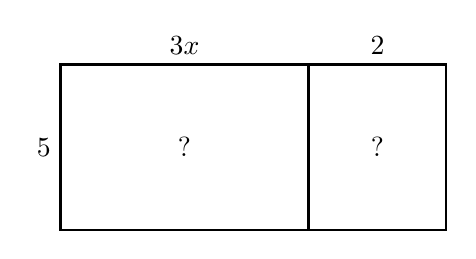
\begin{tikzpicture}[scale=0.7]
  \draw[thick] (0,0) rectangle (7,3);
  \draw[thick] (4.5,0) -- (4.5,3);
  \node[left] at (0,1.5) {$5$};
  \node[above] at (2.25,3) {$3x$};
  \node[above] at (5.75,3) {$2$};
  \node at (2.25,1.5) {?};
  \node at (5.75,1.5) {?};
\end{tikzpicture}
\end{center}
\end{questionText}
\correctAnswer{$15x + 10$}
\explanation{The left section: $5 \times 3x = 15x$. The right section: $5 \times 2 = 10$. Expanded: $5(3x + 2) = 15x + 10$.}
\end{practiceQuestion}

\begin{practiceQuestion}{5-4-q10}{mc}
\begin{questionText}
Solve $\dfrac{x}{6} - \dfrac{2}{3} = \dfrac{1}{2}$.
\end{questionText}
\choiceA{$x = 3$}
\choiceB{$x = 7$}
\choiceC{$x = -1$}
\choiceD{$x = 10$}
\correctAnswer{B}
\explanation{Multiply every term by $6$: $x - 4 = 3$. Add $4$: $x = 7$. Check: $\frac{7}{6} - \frac{2}{3} = \frac{7}{6} - \frac{4}{6} = \frac{3}{6} = \frac{1}{2}$ \checkmark.}
\end{practiceQuestion}

\begin{practiceQuestion}{5-5-q01}{mc}
\begin{questionText}
Solve $2x + 3 > 11$.
\end{questionText}
\choiceA{$x > 4$}
\choiceB{$x > 7$}
\choiceC{$x < 4$}
\choiceD{$x > 14$}
\correctAnswer{A}
\explanation{Subtract $3$: $2x > 8$. Divide by $2$: $x > 4$.}
\end{practiceQuestion}

\begin{practiceQuestion}{5-6-q13}{mc}
\begin{questionText}
True or false: The graph of $x < 5$ and $x \leq 5$ look exactly the same.
\end{questionText}
\choiceA{True — both shade to the left of $5$}
\choiceB{False — $x < 5$ has an open circle, $x \leq 5$ has a closed circle}
\choiceC{False — they shade in different directions}
\choiceD{True — the circle type does not matter}
\correctAnswer{B}
\explanation{$x < 5$ uses an open circle (not including $5$) while $x \leq 5$ uses a closed circle (including $5$). Both shade left.}
\end{practiceQuestion}

\begin{practiceQuestion}{6-1-q02}{mc}
\begin{questionText}
A blueprint uses the scale $1$ in $= 6$ ft. A hallway is $3.5$ in long on the blueprint. What is the actual length?
\end{questionText}
\choiceA{$18$ ft}
\choiceB{$21$ ft}
\choiceC{$24$ ft}
\choiceD{$9.5$ ft}
\correctAnswer{B}
\explanation{$3.5 \times 6 = 21$ ft.}
\end{practiceQuestion}

\begin{practiceQuestion}{6-3-q16}{mc}
\begin{questionText}
A parallelogram has side lengths $5$ cm and $8$ cm. How many different parallelograms can be drawn?
\end{questionText}
\choiceA{None}
\choiceB{Exactly one}
\choiceC{Exactly two}
\choiceD{More than one}
\correctAnswer{D}
\explanation{Two side lengths of a parallelogram do not fix the angles. The shape can be a rectangle, a rhomboid, or anything in between. Many different parallelograms are possible.}
\end{practiceQuestion}

\begin{practiceQuestion}{6-4-q10}{mc}
\begin{questionText}
Can a triangle be formed with sides $7$, $10$, and $15$?
\end{questionText}
\choiceA{No, the triangle inequality fails}
\choiceB{Yes, exactly one triangle}
\choiceC{Yes, more than one triangle}
\choiceD{Yes, but only a right triangle}
\correctAnswer{B}
\explanation{$7 + 10 = 17 > 15$ \checkmark, $7 + 15 = 22 > 10$ \checkmark, $10 + 15 = 25 > 7$ \checkmark. SSS with valid lengths gives one unique triangle.}
\end{practiceQuestion}

\begin{practiceQuestion}{6-5-q07}{mc}
\begin{questionText}
A triangular prism is sliced with a cut parallel to its triangular base. What is the cross-section?
\end{questionText}
\choiceA{A rectangle}
\choiceB{A triangle congruent to the base}
\choiceC{A smaller triangle}
\choiceD{A trapezoid}
\correctAnswer{B}
\explanation{A cut parallel to the base of a prism always produces a shape congruent (same size and shape) to the base. For a triangular prism, this is a triangle identical to the base.}
\end{practiceQuestion}

\begin{practiceQuestion}{6-6-q04}{mc}
\begin{questionText}
Two supplementary angles are $(2x + 10)°$ and $(3x)°$. What is the value of $x$?
\end{questionText}
\choiceA{$30$}
\choiceB{$34$}
\choiceC{$36$}
\choiceD{$40$}
\correctAnswer{B}
\explanation{$2x + 10 + 3x = 180$. Combine: $5x + 10 = 180$. Subtract $10$: $5x = 170$. Divide: $x = 34$.}
\end{practiceQuestion}

\begin{practiceQuestion}{6-7-q09}{mc}
\begin{questionText}
A triangle has vertices $P(1, 2)$, $Q(4, 2)$, and $R(4, 6)$. After a translation, $P' = (3, 0)$. What translation was applied?
\end{questionText}
\choiceA{Right $2$, down $2$}
\choiceB{Left $2$, up $2$}
\choiceC{Right $2$, up $2$}
\choiceD{Left $2$, down $2$}
\correctAnswer{A}
\explanation{From $P(1, 2)$ to $P'(3, 0)$: $x$ changed by $+2$ (right $2$) and $y$ changed by $-2$ (down $2$).}
\end{practiceQuestion}

\begin{practiceQuestion}{7-3-q15}{mc}
\begin{questionText}
A quarter-circle has a radius of $8$ cm. What is its area? Use $\pi \approx 3.14$.
\end{questionText}
\choiceA{$200.96$ cm$^2$}
\choiceB{$100.48$ cm$^2$}
\choiceC{$50.24$ cm$^2$}
\choiceD{$25.12$ cm$^2$}
\correctAnswer{C}
\explanation{Full circle area $= \pi r^2 = 3.14 \times 64 = 200.96$ cm$^2$. Quarter circle $= 200.96 \div 4 = 50.24$ cm$^2$.}
\end{practiceQuestion}

\begin{practiceQuestion}{7-4-q18}{mc}
\begin{questionText}
A pentagon can be divided into a rectangle $6$ cm by $4$ cm and a triangle with base $6$ cm and height $2$ cm. What is the total area?
\end{questionText}
\choiceA{$24$ cm$^2$}
\choiceB{$30$ cm$^2$}
\choiceC{$36$ cm$^2$}
\choiceD{$48$ cm$^2$}
\correctAnswer{B}
\explanation{Rectangle: $6 \times 4 = 24$ cm$^2$. Triangle: $\frac{1}{2} \times 6 \times 2 = 6$ cm$^2$. Total: $24 + 6 = 30$ cm$^2$.}
\end{practiceQuestion}

\begin{practiceQuestion}{7-5-q01}{mc}
\begin{questionText}
What is the surface area of a cube with side length $4$ cm?
\end{questionText}
\choiceA{$16$ cm$^2$}
\choiceB{$64$ cm$^2$}
\choiceC{$96$ cm$^2$}
\choiceD{$24$ cm$^2$}
\correctAnswer{C}
\explanation{A cube has $6$ faces. $SA = 6s^2 = 6 \times 16 = 96$ cm$^2$.}
\end{practiceQuestion}

\begin{practiceQuestion}{7-6-q10}{mc}
\begin{questionText}
A rectangular prism has a base area of $24$ cm$^2$ and a height of $7$ cm. What is its volume?
\end{questionText}
\choiceA{$31$ cm$^3$}
\choiceB{$168$ cm$^3$}
\choiceC{$336$ cm$^3$}
\choiceD{$17$ cm$^3$}
\correctAnswer{B}
\explanation{$V = Bh = 24 \times 7 = 168$ cm$^3$.}
\end{practiceQuestion}

\begin{practiceQuestion}{8-1-q02}{mc}
\begin{questionText}
A researcher wants to know the average height of seventh graders in a state. She measures the heights of $100$ seventh graders from different schools. What is the sample?
\end{questionText}
\choiceA{All seventh graders in the state}
\choiceB{All students in the schools she visited}
\choiceC{The $100$ seventh graders she measured}
\choiceD{The tallest seventh graders}
\correctAnswer{C}
\explanation{The sample is the smaller group chosen from the population — the $100$ students measured.}
\end{practiceQuestion}

\begin{practiceQuestion}{8-3-q26}{gmc}
\begin{questionText}
The box plots below compare test scores for Class A and Class B.

\begin{center}
\begin{tikzpicture}[scale=0.1]
  \draw[thick,->] (49,0) -- (101,0);
  \foreach \x in {50,55,...,100} {
    \draw (\x,0.5) -- (\x,-0.5);
    \node[below,font=\small] at (\x,-0.5) {$\x$};
  }
  % Class A: min=60, Q1=70, med=78, Q3=85, max=95
  \draw[thick] (60,6) -- (95,6);
  \draw[thick,fill=funBlue!30] (70,4) rectangle (85,8);
  \draw[very thick,funBlue] (78,4) -- (78,8);
  \draw[thick] (60,4) -- (60,8);
  \draw[thick] (95,4) -- (95,8);
  \node[right,font=\small] at (96,6) {Class A};
  % Class B: min=50, Q1=58, med=65, Q3=72, max=80
  \draw[thick] (50,14) -- (80,14);
  \draw[thick,fill=funGreen!30] (58,12) rectangle (72,16);
  \draw[very thick,funGreen] (65,12) -- (65,16);
  \draw[thick] (50,12) -- (50,16);
  \draw[thick] (80,12) -- (80,16);
  \node[right,font=\small] at (81,14) {Class B};
\end{tikzpicture}
\end{center}

Which statement is best supported by the box plots?
\end{questionText}
\choiceA{Class B scored higher than Class A}
\choiceB{Class A has a higher median and a larger IQR}
\choiceC{Class A has a higher median and both classes have the same IQR}
\choiceD{Class A and Class B overlap, but Class A's median is higher}
\correctAnswer{D}
\explanation{Class A median $= 78$, Class B median $= 65$. Class A's range ($60$--$95$) overlaps with Class B's range ($50$--$80$), but Class A is higher overall.}
\end{practiceQuestion}

\begin{practiceQuestion}{8-4-q16}{mc}
\begin{questionText}
Group A: $\{60, 65, 70, 75, 80\}$. Group B: $\{40, 55, 70, 85, 100\}$. Both have a mean of $70$. Which group is more variable?
\end{questionText}
\choiceA{Group A}
\choiceB{Group B}
\choiceC{They are equally variable}
\choiceD{Cannot be determined}
\correctAnswer{B}
\explanation{Group A range $= 20$, Group B range $= 60$. Group B's data is far more spread out.}
\end{practiceQuestion}

\begin{practiceQuestion}{8-7-q27}{gmc}
\begin{questionText}
The double bar graph shows the number of goals scored by two soccer teams over four games.

\begin{center}
\begin{tikzpicture}[scale=0.55]
  \draw[thick,->] (0,0) -- (0,6) node[above]{\small Goals};
  \draw[thick,->] (0,0) -- (10,0);
  % Game 1
  \fill[funBlue!70] (0.5,0) rectangle (1.2,3);
  \fill[funGreen!70] (1.3,0) rectangle (2.0,2);
  \node[below,font=\tiny] at (1.25,0) {G1};
  % Game 2
  \fill[funBlue!70] (2.5,0) rectangle (3.2,4);
  \fill[funGreen!70] (3.3,0) rectangle (4.0,5);
  \node[below,font=\tiny] at (3.25,0) {G2};
  % Game 3
  \fill[funBlue!70] (4.5,0) rectangle (5.2,2);
  \fill[funGreen!70] (5.3,0) rectangle (6.0,3);
  \node[below,font=\tiny] at (5.25,0) {G3};
  % Game 4
  \fill[funBlue!70] (6.5,0) rectangle (7.2,5);
  \fill[funGreen!70] (7.3,0) rectangle (8.0,4);
  \node[below,font=\tiny] at (7.25,0) {G4};
  \foreach \y in {1,...,5} { \draw (-0.1,\y) -- (0.1,\y); \node[left,font=\tiny] at (0,\y) {$\y$}; }
  % legend
  \fill[funBlue!70] (8.5,5) rectangle (9,5.3);
  \node[right,font=\tiny] at (9,5.15) {Team A};
  \fill[funGreen!70] (8.5,4.3) rectangle (9,4.6);
  \node[right,font=\tiny] at (9,4.45) {Team B};
\end{tikzpicture}
\end{center}

Which team scored more total goals?
\end{questionText}
\choiceA{Team A with $14$ goals}
\choiceB{Team B with $14$ goals}
\choiceC{They tied with $14$ goals each}
\choiceD{Team A with $12$ goals}
\correctAnswer{C}
\explanation{Team A: $3+4+2+5 = 14$. Team B: $2+5+3+4 = 14$. They tied.}
\end{practiceQuestion}

\begin{practiceQuestion}{9-4-q09}{mc}
\begin{questionText}
A teacher predicted that a spinner would land on red $\frac{1}{4}$ of the time. After $80$ spins, red appeared $25$ times. How do the observed and predicted results compare?
\end{questionText}
\choiceA{They are very different — the model is wrong}
\choiceB{The observed ($\frac{25}{80} = 0.3125$) is close to the predicted ($0.25$)}
\choiceC{The observed result is exactly equal to the predicted result}
\choiceD{The predicted probability is higher than the observed}
\correctAnswer{B}
\explanation{Predicted: $\frac{1}{4} = 0.25$. Observed: $\frac{25}{80} = 0.3125$. They are close, which supports the model.}
\end{practiceQuestion}

\begin{practiceQuestion}{9-6-q18}{mc}
\begin{questionText}
Three coins are flipped. What is the probability of getting NO heads (all tails)?
\end{questionText}
\choiceA{$\frac{1}{2}$}
\choiceB{$\frac{1}{4}$}
\choiceC{$\frac{1}{8}$}
\choiceD{$\frac{3}{8}$}
\correctAnswer{C}
\explanation{Only one outcome out of $8$ is all tails (TTT). $P = \frac{1}{8}$.}
\end{practiceQuestion}

\begin{practiceQuestion}{9-7-q24}{sa}
\begin{questionText}
Describe how to use a standard die to simulate a $\frac{1}{3}$ probability event.
\end{questionText}
\correctAnswer{Roll the die; let $1$ and $2$ represent the event (or any $2$ numbers out of $6$)}
\explanation{Choose $2$ of the $6$ faces to represent the event. $P = \frac{2}{6} = \frac{1}{3}$.}
\end{practiceQuestion}
